\begin{frame}[fragile]
        \frametitle{Pulsed Nuclear Magnetic Resonance}
        \begin{center}
              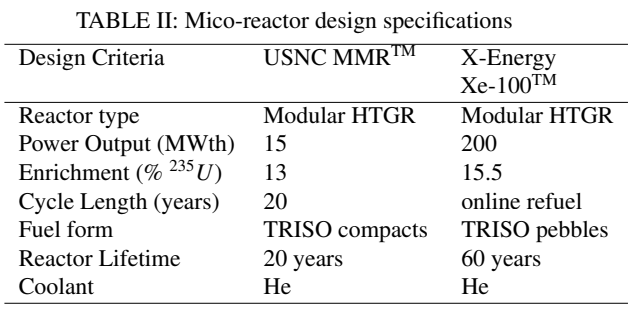
\includegraphics[height=5cm]{./images/specifications.png}
      \end{center}
\end{frame}

\begin{frame}
  \frametitle{Fuel}
  % a comment
        \begin{columns}
                \column[t]{5cm}
                \begin{itemize}
                        \item TRIstructural ISOtropic fuel has core of uranium, carbon, and oxygen: and is coated in layers of ceramic
                        \item Roughly the size of billiard balls
                        \item Load follows
                        \item Fuel transitions directly to dry-cask storage
                \end{itemize}

                \column[t]{5cm}
        \begin{figure}[htbp!]
        \begin{center}
      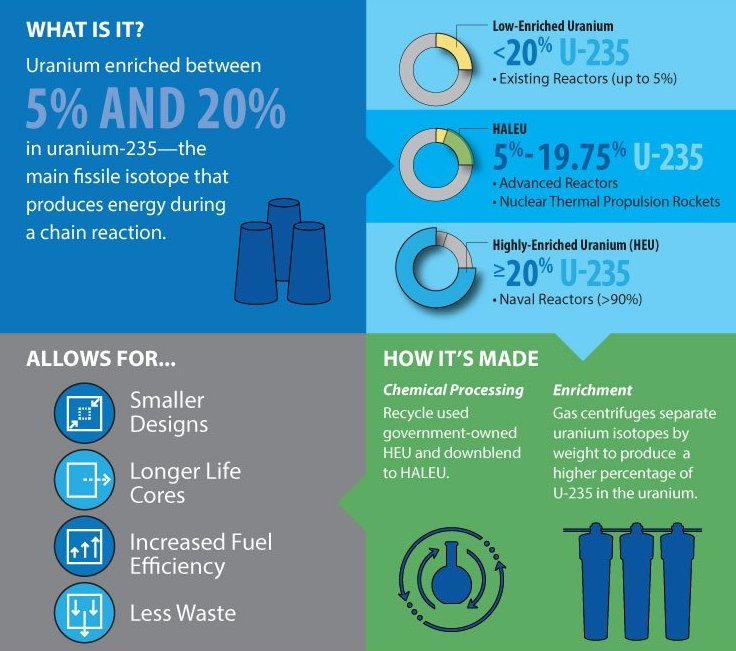
\includegraphics[height=4cm]{./images/HALEU_overview.jpg}
    \end{center}
          \caption{DOE HALEU Overview}
    \label{fig:doe_haleu_overview}
  \end{figure}
        \end{columns}
\end{frame}

